\documentclass[11pt,a4paper]{article}

% ------------------------
% Packages
% ------------------------
\usepackage[utf8]{inputenc}
\usepackage[T1]{fontenc}
\usepackage{lmodern}

\usepackage{geometry}
\geometry{margin=2.5cm}

\usepackage{setspace}
\onehalfspacing

\usepackage{graphicx}
\usepackage{amsmath, amssymb}

\usepackage{booktabs}
\usepackage{array}
\usepackage{multirow}

\usepackage{hyperref}
\hypersetup{
    colorlinks=true,
    linkcolor=black,
    citecolor=black,
    urlcolor=black
}

\usepackage{caption}
\usepackage{subcaption}

\usepackage{enumitem}
\usepackage{multicol}
\usepackage{blindtext}
\usepackage{pgfplots}
\pgfplotsset{compat=1.18}
\usepackage{tikz}
\usetikzlibrary{positioning,calc}

% Chart colours for the three configurations compared with the static pipeline
\definecolor{cleaning}{HTML}{2A78D6}
\definecolor{metaonly}{HTML}{EB6834}
\definecolor{fullsystem}{HTML}{1BAF7A}

% Floats do not work inside multicols; tables there are placed in the text flow
\newenvironment{coltable}{\par\medskip\noindent\begin{minipage}{\linewidth}\centering\small}{\end{minipage}\par\medskip}

% ------------------------
% Title Information
% ------------------------
\title{\textbf{Intelligent Automation of Data Preparation Using Meta-Learning and Performance-Driven Optimization}}

\author{
    Parinaz Teimouri \\
    Applied Computer Science \\
    FH Schmalkalden University of Applied Sciences \\
    \texttt{p.teimouri@stud.fh-sm.de}
}

\date{\today}

% ------------------------
% Document
% ------------------------
\begin{document}
\maketitle

% ---------------- ABSTRACT ----------------
\begin{abstract}
Data preparation remains one of the most time-intensive aspects of machine learning projects, often requiring considerable manual effort and domain expertise. While automated machine learning has advanced, data preprocessing still relies heavily on fixed rules that do not adapt to specific dataset characteristics. This paper presents an automated approach to data preparation that repairs inconsistent values, keeps the column to be predicted out of all preprocessing, and selects preprocessing strategies based on measured performance rather than predetermined heuristics. Strategies for missing values and feature scaling are shortlisted by meta-learning and then tested with a downstream model; categorical encoding and outlier handling adapt to the statistics of each column. Every decision is logged, so the process remains transparent and reproducible. In a benchmark on seven datasets with five random splits each, the system outperformed a fixed preprocessing pipeline in 28 of 35 paired comparisons. Most of this gain came from the automatic repair of values; testing strategies against the target added little over good fixed defaults. The paper also discusses current limitations and potential directions for future research.
\end{abstract}

\noindent\textbf{Keywords:} Automated Data Preparation, Meta-Learning, Tabular Data, Machine Learning Pipelines, Feature Engineering


\section*{Benchmark at a Glance}

Figure~\ref{fig:comparison} summarises the benchmark reported in Section~\ref{sec:results}. Seven datasets were prepared in four ways and scored with two downstream models over five random splits. The figure shows how much each configuration improves on a static pipeline that uses mean imputation, one-hot encoding and standard scaling without any value cleaning.

\begin{figure}[h]
\centering
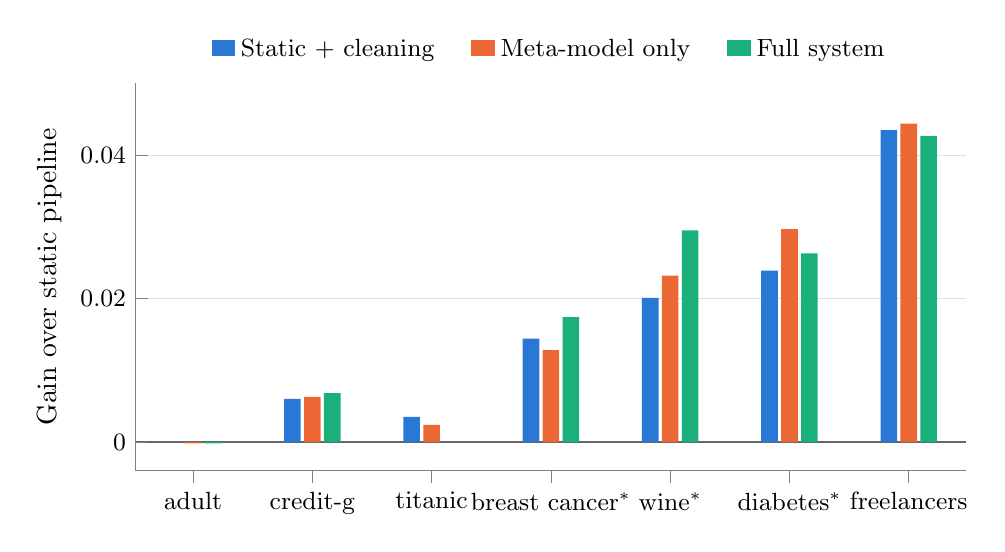
\begin{tikzpicture}
\begin{axis}[
    width=\linewidth,
    height=6.5cm,
    ybar=1.2pt,
    bar width=6pt,
    ymin=-0.004, ymax=0.05,
    scaled y ticks=false,
    ylabel={Gain over static pipeline},
    symbolic x coords={adult, creditg, titanic, breast, wine, diabetes, freelancers},
    xtick=data,
    xticklabels={adult, credit-g, titanic, breast cancer$^\ast$, wine$^\ast$, diabetes$^\ast$, freelancers},
    x tick label style={font=\small},
    y tick label style={font=\small, /pgf/number format/fixed, /pgf/number format/precision=2},
    ymajorgrids,
    major grid style={black!12},
    axis x line*=bottom,
    axis y line*=left,
    axis line style={black!50},
    tick style={black!50},
    enlarge x limits=0.08,
    extra y ticks={0},
    extra y tick labels={},
    extra y tick style={grid=major, major grid style={black!60}},
    legend style={at={(0.5,1.03)}, anchor=south, legend columns=-1, draw=none, font=\small,
                  /tikz/every even column/.append style={column sep=0.4cm}},
    legend image code/.code={\fill[#1] (0cm,-0.08cm) rectangle (0.3cm,0.12cm);},
]
\addplot[fill=cleaning, draw=none] coordinates {
    (adult,0.0000) (creditg,0.0060) (titanic,0.0035) (breast,0.0144) (wine,0.0201) (diabetes,0.0239) (freelancers,0.0435)};
\addplot[fill=metaonly, draw=none] coordinates {
    (adult,-0.0002) (creditg,0.0063) (titanic,0.0024) (breast,0.0128) (wine,0.0232) (diabetes,0.0297) (freelancers,0.0444)};
\addplot[fill=fullsystem, draw=none] coordinates {
    (adult,-0.0002) (creditg,0.0068) (titanic,0.0000) (breast,0.0174) (wine,0.0295) (diabetes,0.0263) (freelancers,0.0427)};
\legend{Static + cleaning, Meta-model only, Full system}
\end{axis}
\end{tikzpicture}
\caption{Mean gain in downstream score (macro F1 for classification, $R^2$ for regression) over the static pipeline. Real OpenML datasets on the left, datasets with defects on the right ($^\ast$ = defects injected, freelancers = messy as delivered). The gain appears wherever values need cleaning, and the three configurations that clean are close together.}
\label{fig:comparison}
\end{figure}

The benchmark leads to four main observations:

\begin{itemize}
    \item \textbf{Cleaning drives the gain:} Repairing values and leaving ID columns out improves on the static pipeline in 24 of 35 paired comparisons, by 0.016 on average.
    \item \textbf{Testing strategies adds little:} Choosing imputation and scaling by cross-validated evaluation adds 0.002 over good fixed defaults (18 wins, 5 ties, 12 losses).
    \item \textbf{Gains depend on the data:} Improvements reach up to 0.04 on datasets with defects, while on clean real data all configurations lie within 0.007 of each other.
    \item \textbf{Low cost:} The full system needed 0.36 seconds per run on average on the benchmark datasets (up to 3,000 rows), compared with 0.17 seconds for the static pipeline.
\end{itemize}


\setlength{\columnsep}{0.8cm}
\setlength{\columnseprule}{0.4pt}
\begin{multicols}{2}

% ---------------- BACKGROUND ----------------
\section{Scientific Background and Related Knowledge}

Machine learning models perform best when working with clean, well-prepared data. However, real-world datasets often arrive with various issues including missing values, mixed formats, outliers, and different types of features. Research indicates that data preparation can consume up to 80\% of the time in machine learning projects, making it a significant bottleneck in the development process [2].

Most current data preprocessing approaches rely on predetermined rules applied universally across datasets. Common practices include replacing missing numerical values with the mean or median, and converting categorical variables using one-hot encoding. While these methods work in some situations, they don't account for the unique characteristics of individual datasets. This one-size-fits-all approach can lead to suboptimal results when dealing with diverse data distributions and varying data quality issues [1, 9].

Automated Machine Learning (AutoML) systems have made progress in reducing manual work by handling model selection and parameter tuning automatically. However, many of these systems either expect data to be preprocessed beforehand or apply basic preprocessing rules without considering what might work best for the specific dataset at hand. This leaves data preparation as a largely manual task that requires significant expertise and time investment.

Recent work has begun exploring how meta-learning might help address these challenges. Meta-learning involves learning from experience with previous datasets to make better decisions on new data. The idea is to identify patterns between dataset characteristics and successful preprocessing strategies. While this research direction shows promise, many existing approaches focus on individual preprocessing steps in isolation and don't always validate their choices using actual model performance.

This research takes a practical approach by focusing on preprocessing decisions that demonstrably improve model performance. Rather than relying solely on theoretical considerations or fixed rules, the system evaluates different preprocessing options based on how well they help downstream models perform on the specific task at hand.


\subsection{Limitations of Rule-Based Data Preparation}

Most practical machine learning systems still rely on predetermined preprocessing rules applied uniformly across datasets. These approaches use fixed thresholds and assumptions, such as always replacing missing values with the mean or using one-hot encoding for categorical variables. While simple to implement, they assume all datasets share similar statistical properties, which rarely holds true.

Static rules often fail to adapt to specific data distributions; for instance, mean imputation can introduce bias in skewed data, while one-hot encoding may lead to dimensionality issues with high-cardinality features. Furthermore, isolated preprocessing choices often ignore potential interactions between steps. Relying on convention rather than empirical evidence frequently results in suboptimal pipelines, highlighting the need for adaptive systems.

\subsection{Data Preparation as an Optimization Problem}

Data preparation can be viewed as finding the best sequence of preprocessing steps that leads to optimal model performance. Consider a raw dataset $D$ and various preprocessing pipelines $p$ that can transform it into different processed versions $D_p$. Each processed dataset can then be used to train a machine learning model $M$.

The goal is to find the preprocessing pipeline $p^*$ that produces the best model performance:

\[
p^* = \arg\max_{p \in \mathcal{P}} J(M(D_p))
\]

where $J$ represents a performance metric appropriate for the task.

This perspective treats preprocessing as an integral part of the machine learning pipeline rather than a separate preliminary step. However, the number of possible preprocessing combinations grows rapidly with each additional step and strategy option, making exhaustive search impractical. Therefore, practical approaches need to use intelligent strategies to navigate this large search space efficiently. The proposed system addresses this challenge by making locally optimal decisions at each preprocessing stage based on empirical evaluation of their impact on model performance.


% ---------------- OPEN TOPIC ----------------
\section{Selected Open Topic}

This research focuses on developing an automated system for data preparation that can adapt to different types of tabular datasets. The work addresses three main challenges:

\begin{itemize}
    \item Selecting preprocessing strategies based on dataset characteristics rather than fixed rules
    \item Evaluating preprocessing quality using objective performance metrics
    \item Maintaining transparency and reproducibility while automating the process
\end{itemize}

These challenges remain difficult due to the complexity of preprocessing decisions and the large number of possible preprocessing combinations. Rather than attempting to find a globally optimal solution, this research explores a practical approach that identifies effective local strategies at each preprocessing step while balancing performance, interpretability, and computational efficiency.

% ---------------- METHODS ----------------
\section{Methods}

\subsection{System Architecture}

The proposed system is implemented as a modular Python pipeline with a central \texttt{AutoDataPreparer} class that coordinates different preprocessing tasks. Each preprocessing step is handled separately, facilitating the extension or modification of individual components. The steps run in this order:

\begin{enumerate}[noitemsep, leftmargin=*]
    \item Load the file (CSV in any common encoding and delimiter, or Excel)
    \item Set the target column aside
    \item Repair inconsistent values
    \item Detect the task type
    \item Parse dates
    \item Remove duplicate rows
    \item Leave ID and free-text columns out
    \item Cap rare outliers
    \item Fill missing values
    \item Encode categories
    \item Scale numbers
\end{enumerate}

The system writes two files: a human-readable one after step 9, which keeps the ID columns and the original values, and an ML-ready one after step 11. Values are repaired before duplicates are removed, so that rows differing only in spelling are recognised as duplicates.

\subsection{Target Separation}

The column to be predicted is removed from the data before any other step and only added back when the results are written. This way, no preprocessing step can change it, and the evaluation of candidate strategies cannot use it as an input, which would make the results look better than they are. Rows without a target value are dropped, as they cannot be used for evaluation. The target receives the same value repairs as the other columns, but it is never filled in or scaled.

\subsection{Value Standardisation}

Real exports often contain the same information written in different ways. The system checks every text column for three kinds of problems and repairs the first one that applies:

\begin{itemize}[leftmargin=*]
    \item \textbf{Yes/no text:} columns that only contain values such as yes/no, Y/N, True/False, 1/0 or the German ja/nein become 0/1.
    \item \textbf{Numbers stored as text:} currency signs and percent signs are removed, and German and English number formats are recognised (``89,90~\texteuro'', ``1.299,00'', ``EUR 1,299.00'', ``84\%''). If at least 90\% of the values can be read, the column becomes numeric.
    \item \textbf{Different spellings:} values that differ only in capitalisation or spaces are merged (``NAVY'', ``navy'', ``Navy''). In columns with at most ten categories, a single letter is merged with the only longer value that starts with it (``m'' becomes ``male'').
\end{itemize}

Columns named like IDs are left exactly as they are.

\subsection{Identifier Detection}

ID columns and free text describe single rows and do not help a model learn general patterns; one-hot encoding them only creates thousands of useless columns. The system therefore leaves out text columns in which at least 95\% of the values are unique, and columns named like an ID (for example \emph{id}, \emph{sku} or \emph{invoice no}) that have many different values. A store ID with five stores is still treated as a normal category. The excluded columns remain in the human-readable file.

\subsection{Task Type Detection}

The system then identifies whether the prediction task involves classification or regression by examining the target variable. Text targets are treated as classification problems. Numeric targets with decimal values, such as a rating of 3.3, are treated as regression, while whole-number targets with fewer than 20 distinct values (or fewer than 5\% distinct values) are treated as classification. This enables the system to choose appropriate evaluation metrics and models for the specific problem type.

\subsection{Meta-Feature Extraction}

For each decision, the system describes one column with a few simple statistics (Table~\ref{tab:meta}): for missing values the column with the most gaps, for scaling the most skewed column, and for encoding each categorical column. These simple metrics help the system make informed preprocessing decisions based on established meta-learning approaches [5].

\begin{coltable}
\captionof{table}{Extracted Meta-Features}
\label{tab:meta}
\begin{tabular}{ll}
\toprule
\textbf{Meta-Feature} & \textbf{Description} \\
\midrule
Rows & Size of the dataset \\
Missing Ratio & Share of missing values \\
Skewness & Distribution asymmetry \\
Kurtosis & Tail heaviness \\
Unique Ratio & Share of distinct values \\
Data Type & Numeric or categorical \\
\bottomrule
\end{tabular}
\end{coltable}

\subsection{Missing Value Imputation}

The system treats missing value handling as a choice between different strategies rather than applying a fixed rule. For numerical features, it considers mean imputation, median imputation, and K-nearest neighbors imputation. Columns that only contain 0 and 1 are filled with their most common value instead, since a value such as 0.67 is not a valid yes/no flag.

For categorical features with only a few gaps, the most frequent category is used. If more than 10\% of a column is missing, or the column has more than 50 different values, the gaps are marked as \texttt{(missing)} instead, because copying one common value into many rows would invent information. Research shows that imputation choices can significantly affect final model accuracy [1, 10].


\subsection{Categorical Encoding}

The system handles categorical features by choosing between one-hot encoding and label encoding for each column, based on its statistics. Without a trained meta-model, columns in which fewer than 5\% of the values are distinct use one-hot encoding, and all others use label encoding to avoid creating too many features [1]. Unlike missing values and scaling, the encoding is predicted but not tested against the target.


\subsection{Feature Scaling}

The system selects scaling methods for numerical features based on their impact on model performance. It considers standardization, min-max scaling, and robust scaling. Since tree-based models are not affected by the scale of a feature, the scaling options are tested with a K-nearest neighbors model, which is.


\subsection{Outlier Detection and Treatment}

The system handles outliers using a practical approach that balances data preservation with noise reduction. The process has two steps: identifying potential outliers and deciding how to treat them.

\subsubsection{Detection Mechanism}
The Interquartile Range (IQR) method is employed for efficient outlier identification. The system flags values that fall outside the range $[Q_1 - 1.5 \times \text{IQR}, Q_3 + 1.5 \times \text{IQR}]$ [2].

\subsubsection{Adaptive Treatment}
After identifying potential outliers, the system determines the appropriate handling method based on their frequency:

\begin{itemize}
    \item \textbf{Low Outlier Frequency ($< 5\%$):} When outliers are rare, the system applies Winsorization by capping extreme values at the IQR boundaries. This reduces the influence of extreme values while retaining all data points.
    \item \textbf{High Outlier Frequency ($\geq 5\%$):} When outliers are common, the system preserves the original values, recognizing that the feature may naturally exhibit a heavy-tailed distribution containing relevant information for prediction.
\end{itemize}

The capping is only applied to the ML-ready file. The human-readable file keeps the original values, so a genuinely high price is never changed in the file a person reads.


\subsection{Decision Transparency}

The system maintains a record of all preprocessing decisions through a logging mechanism. It generates a detailed report showing each transformation applied to the data, including the specific method used, how many data points were affected, the scores of the tested strategies, how many rows were removed and why, and the time taken by each step. This logging ensures that the automated process remains transparent and reproducible, allowing users to understand exactly what changes were made to their data.

\subsection{Top-K Strategy Selection}

To balance performance with computational efficiency, the system uses a two-phase approach to select strategies for missing values and scaling:
\begin{itemize}
    \item \textbf{Phase 1: Initial filtering.} Based on the column statistics, the meta-learner ranks the candidate strategies and keeps the top $k$ (currently $k=2$). Without a trained meta-model, the fixed rule's choice comes first.
    \item \textbf{Phase 2: Performance testing.} Each candidate is tested inside a complete preprocessing and model pipeline with 3-fold cross-validation: with a random forest (50 trees) for missing values and with K-nearest neighbors for scaling.
    \item \textbf{Selection.} The strategy with the best result (highest macro F1-score for classification or $R^2$ for regression) is selected and stored as feedback for future training. This approach combines learned knowledge with practical validation [4, 6, 7].
\end{itemize}


\subsection{Meta-Model Training}

The meta-learner is a random forest classifier for each task that predicts the best strategy from the column statistics. It learns from measured results rather than hand-written labels: a training script creates synthetic datasets of different sizes, shapes and noise levels, adds skewed columns, missing values or categories, and tests every strategy on each dataset in the same way the pipeline does. The strategy that scores best becomes the label. Results from real pipeline runs are added to the training data over time.


\subsection{Pipeline Decision Flow}

The preprocessing pipeline processes data sequentially, with each step building on the output of the previous one. This approach mirrors how data scientists typically work and ensures compatibility with standard machine learning tools.

At the tested stages, the system defines a small set of candidate strategies and evaluates them empirically. Rather than relying solely on theoretical considerations, it trains a model to test how well each preprocessing approach works with the specific dataset.

To keep computational costs reasonable, the evaluation uses small models (a random forest with 50 trees, or K-nearest neighbors). Whether their judgement carries over to other models is not guaranteed, which is why the benchmark scores the results with two different models.

\subsection{Computational Complexity Considerations}

Testing different preprocessing strategies adds computational overhead compared to using fixed rules. For each tested stage with $k$ candidate strategies and $n$ data samples, the complexity is approximately:

\[
\mathcal{O}(k \cdot T_{model}(n))
\]

where $T_{model}(n)$ is the time to train the evaluation model. To manage this cost, the system tests only two candidates and excludes expensive options for large datasets: K-nearest neighbors imputation is skipped above 10,000 rows because its cost grows quadratically with the number of rows.

\subsection{Automated Feature Engineering and Type Enforcement}

The system includes additional features for handling temporal data and maintaining data consistency. It detects date columns by testing whether their values look like dates and can be parsed, reading dates written with dots (``01.12.2010'') day-first as is usual in Germany. It then extracts year, month, and day to help capture seasonal patterns. Columns that originally held only whole numbers, such as ages or counts, are rounded back to whole numbers after missing values have been filled.


% ---------------- RESULTS ----------------
\section{Results}
\label{sec:results}

\subsection{Experimental Setup}

The system was tested on seven datasets: three scikit-learn datasets (breast cancer, wine, diabetes) with added defects typical of real exports (missing values, skewed columns, numbers stored as currency text, a category in four spellings, a yes/no column in mixed notation and an ID column); a messy freelancer export from the repository; and three real OpenML datasets used as they are (Titanic, adult census and German credit).

Four configurations were compared:
\begin{itemize}[leftmargin=*, noitemsep]
    \item \textbf{Static:} mean imputation, one-hot encoding, standard scaling, no value cleaning
    \item \textbf{Static + cleaning:} the same, plus value repair and ID removal
    \item \textbf{Meta-model only:} cleaning, with strategies predicted but not tested
    \item \textbf{Full system:} cleaning, with the two best candidates tested against the target
\end{itemize}

Each dataset was split into two halves, five times with different random splits. The full system chose its strategies on one half and was scored on the other, so it was never scored on the rows it was tuned on. Each result was scored with a linear model and a random forest using 5-fold cross-validation (macro F1 for classification, $R^2$ for regression), and the two scores were averaged.

\subsection{Downstream Performance}

Table~\ref{tab:results} shows the mean scores. The static pipeline has the worst mean rank; the three configurations that clean the values are close together. The largest gains appear on the datasets with defects, while on the three real OpenML datasets all configurations lie within 0.007 of each other. On the freelancer data every configuration scores below zero, which means the rating is barely predictable from the other columns; cleaning still reduces the error.

\begin{coltable}
\captionof{table}{Mean score over five splits (best per row in bold; $^\ast$ = defects added)}
\label{tab:results}
\setlength{\tabcolsep}{1.8pt}
\begin{tabular}{lcccc}
\toprule
\textbf{Dataset} & \textbf{Static} & \textbf{+Clean} & \textbf{Meta} & \textbf{Full} \\
\midrule
adult & \textbf{0.772} & \textbf{0.772} & 0.772 & 0.772 \\
breast cancer$^\ast$ & 0.936 & 0.950 & 0.949 & \textbf{0.953} \\
credit-g & 0.661 & 0.667 & 0.668 & \textbf{0.668} \\
diabetes$^\ast$ & 0.280 & 0.304 & \textbf{0.309} & 0.306 \\
freelancers & $-$0.155 & $-$0.111 & \textbf{$-$0.111} & $-$0.112 \\
titanic & 0.777 & \textbf{0.781} & 0.779 & 0.777 \\
wine$^\ast$ & 0.941 & 0.961 & 0.964 & \textbf{0.971} \\
\midrule
Mean rank & 3.50 & 2.21 & \textbf{2.07} & 2.21 \\
\bottomrule
\end{tabular}
\end{coltable}

Cleaning also keeps the data compact: the static pipeline one-hot encodes ID and text columns and creates up to 1,543 features, while the full system keeps 11 to 90.

\subsection{Ablation Study}

Since every configuration is scored on the same split, each dataset and split gives one paired comparison, 35 in total (Table~\ref{tab:ablation}).

\begin{coltable}
\captionof{table}{Paired comparisons (7 datasets $\times$ 5 splits)}
\label{tab:ablation}
\setlength{\tabcolsep}{4pt}
\begin{tabular}{lcccc}
\toprule
\textbf{Comparison} & \textbf{W} & \textbf{T} & \textbf{L} & \textbf{Diff.} \\
\midrule
Cleaning vs.\ static & 24 & 5 & 6 & +0.016 \\
Full vs.\ cleaning & 18 & 5 & 12 & +0.002 \\
Full vs.\ meta-model & 10 & 17 & 8 & +0.001 \\
Full vs.\ static & 28 & 0 & 7 & +0.018 \\
\bottomrule
\end{tabular}
\end{coltable}

Cleaning the values accounts for about 90\% of the total gain. Testing strategies against the target wins slightly more often than it loses, but its average advantage of 0.002 is much smaller than the variation between splits. In 17 of 35 cases, testing simply confirmed the predicted strategy.

\subsection{Meta-Model Accuracy}

To check whether column statistics predict the best strategy, meta-models were trained on 150 synthetic datasets per task and cross-validated (Table~\ref{tab:hits}).

\begin{coltable}
\captionof{table}{Share of datasets where the best strategy is ranked first (top-1) or among the two tested candidates (top-2)}
\label{tab:hits}
\setlength{\tabcolsep}{4pt}
\begin{tabular}{lccc}
\toprule
 & \textbf{Imput.} & \textbf{Scaling} & \textbf{Encod.} \\
\midrule
Majority guess & 0.44 & 0.69 & 0.69 \\
Rules, top-1 & 0.25 & 0.65 & 0.41 \\
Model, top-1 & 0.46 & 0.67 & 0.66 \\
Rules, top-2 & 0.57 & 0.80 & 1.00 \\
Model, top-2 & \textbf{0.73} & \textbf{0.84} & 1.00 \\
\bottomrule
\end{tabular}
\end{coltable}

As a single guess, the trained meta-model is hardly better than always picking the most common strategy, and slightly worse for scaling and encoding. As a shortlist of two, it finds the best imputation strategy in 73\% of cases, compared with 57\% for the fixed rules. Using the trained meta-models in the benchmark did not improve the results.

\subsection{Key Advantages}

The proposed system offers several practical benefits compared to traditional preprocessing approaches:
\begin{itemize}
    \item \textbf{Automatic value repair:} Inconsistent spellings, numbers stored as text and yes/no columns are fixed without manual work. This is the step with the largest measured effect.
    \item \textbf{Fair evaluation:} The target is kept out of all preprocessing, and strategies are tested on different rows than the ones they are scored on.
    \item \textbf{Data preservation during outlier handling:} Rather than removing outlier rows, which can introduce bias, the system uses Winsorization to cap extreme values while retaining the complete dataset, and the human-readable file keeps the original values.
    \item \textbf{Adaptation to data characteristics:} The system recognizes when outliers represent natural variation versus noise and adjusts its treatment accordingly, avoiding the uniform application of rigid rules.
    \item \textbf{Transparency:} The system generates detailed documentation of all applied transformations, facilitating the understanding and reproducibility of the preprocessing pipeline.
\end{itemize}


\section{Discussion}

The results show that automating data preparation pays off, but mainly through value repair: fixing spellings, number formats and ID columns improves results clearly, while choosing between imputation and scaling strategies changes little on these datasets. The candidate strategies usually perform within the noise of one another, which also explains why neither the fixed rules nor the trained meta-model predicts the best one reliably. Testing against the target is still useful as a safeguard, because it measures instead of assuming, and it costs only a fraction of a second.

The benchmark has limitations: it covers seven datasets, and the defects in three of them were added synthetically, which favours the cleaning step. The meta-features describe a single column, and the meta-models were trained on synthetic data only.

The current approach makes local optimization decisions at each preprocessing stage rather than searching for a globally optimal combination. While this keeps computational costs manageable, it may miss interactions between different preprocessing steps. For instance, the best encoding method might depend on which scaling approach is used. Handling such dependencies remains a challenge for future work.

Another consideration is computational cost, particularly for large datasets. While the system uses strategies to reduce this burden, the evaluation-based approach may not be suitable for real-time applications or environments with limited computing resources. Combining meta-learning with pre-computed knowledge could help address this limitation.


% ---------------- OPEN QUESTIONS ----------------
\section{Future Work}

Several areas remain for future development:

\begin{itemize}
    \item \textbf{Global pipeline optimization:} Currently, the system optimizes each preprocessing step independently. Future work could explore joint optimization of the entire preprocessing pipeline.
    \item \textbf{Richer meta-features:} Describing the whole dataset and the relationship between columns and target, instead of a single column, may make strategy prediction more reliable.
    \item \textbf{Real training data:} Training the meta-models on real datasets in addition to synthetic ones.
    \item \textbf{Larger benchmark:} More real, messy datasets would allow cleaning to be evaluated without added defects.
    \item \textbf{Advanced strategy selection:} Reinforcement learning approaches could potentially improve how the system selects preprocessing strategies.
    \item \textbf{Broader data types:} Extending the approach to handle non-tabular data such as images, text, or multimodal datasets presents interesting challenges.
\end{itemize}

% ---------------- LITERATURE ----------------
\section{Literature}

This paper intentionally omits formal literature citations in accordance with the assignment requirements. Nevertheless, the proposed framework builds upon established concepts in meta-learning, automated machine learning, and performance-driven optimization.


\begin{thebibliography}{99}

\bibitem{kuhn2019feature}
M. Kuhn and K. Johnson,
\textit{Feature Engineering and Selection: A Practical Approach for Predictive Models},
CRC Press, 2019.

\bibitem{garcia2015data}
S. Garcia, J. Luengo, and F. Herrera,
\textit{Data Preprocessing in Data Mining},
Springer, 2015.

\bibitem{bilalli2017automated}
B. Bilalli, A. Abelló, and T. Aluja-Banet,
``Automated data preprocessing for Big Data,''
\textit{Proceedings of the International Conference on Big Data Analytics}, 2017.

\bibitem{he2019automl}
X. He, K. Zhao, and X. Chu,
``AutoML: A survey of the state-of-the-art,''
\textit{Knowledge-Based Systems}, vol. 212, 2021.

\bibitem{vanschoren2019metalearning}
J. Vanschoren,
``Meta-learning: A survey,''
\textit{Foundations and Trends in Machine Learning},
vol. 11, no. 1, pp. 1--224, 2019.

\bibitem{feurer2015efficient}
M. Feurer et al.,
``Efficient and robust automated machine learning,''
\textit{Advances in Neural Information Processing Systems (NeurIPS)}, 2015.

\bibitem{zoller2021survey}
M.-A. Zöller and M. F. Huber,
``Benchmark and survey of automated machine learning frameworks,''
\textit{Journal of Artificial Intelligence Research}, vol. 70, pp. 409--472, 2021.

\bibitem{bergstra2012random}
J. Bergstra and Y. Bengio,
``Random search for hyper-parameter optimization,''
\textit{Journal of Machine Learning Research}, vol. 13, pp. 281--305, 2012.

\bibitem{guyon2006feature}
I. Guyon and A. Elisseeff,
``An introduction to variable and feature selection,''
\textit{Journal of Machine Learning Research}, vol. 3, pp. 1157--1182, 2003.

\bibitem{domingos2012few}
P. Domingos,
``A few useful things to know about machine learning,''
\textit{Communications of the ACM}, vol. 55, no. 10, pp. 78--87, 2012.

\end{thebibliography}


\end{multicols}
\end{document}
